\documentclass[a4paper, 12pt]{article}

% Permette di scrivere tutti i caratteri unicode senza formule strane
\usepackage[utf8]{inputenc}
\usepackage{textcomp}
\usepackage{multirow}
\usepackage{float}
%\usepackage[caption = false]{subfig}

%Per andare a capo fra pagine con le tabelle
\usepackage{longtable}

%Per inserire codice
\usepackage{listings}

%Cose di matematica
\usepackage{mathtools}
\usepackage{commath}

%Per fare l'1 bbold della matrice identità
\usepackage{bbold}
\usepackage{xcolor}

%Utilissimo per il formalismo della meccanica quantistica, matrici,
%parentesi che si ridimensionano...
\usepackage{physics}

%Ridimensiona i margini
\usepackage[margin=1.8cm]{geometry}

%Etichette per le sotto-immagini
\usepackage{caption}
\usepackage{subcaption}

%Blocchi colorati
\usepackage{mdframed}
\allowdisplaybreaks

%
\numberwithin{equation}{section}
\usepackage[perpage]{footmisc}


\usepackage{cprotect}

\usepackage{tikz-cd}
\usepackage{amsmath}
\usepackage{amsfonts}
\usepackage{amssymb}
\usepackage{amsthm}
\usepackage{graphicx}
%\usepackage[colorinlistoftodos]{todonotes}
\usepackage[colorlinks=true, allcolors=blue, breaklinks=true]{hyperref}
\usepackage{etoolbox}
\appto\UrlBreaks{\do\-}
\usepackage{nameref}
\usepackage[version=4]{mhchem}
\usepackage{siunitx}
\sisetup{separate-uncertainty=true}
\usepackage{cancel}

%%
%Comandi per le frazioni semi-inline
%%

\usepackage{nicefrac}
\usepackage{ifthen}
\let\oldfrac\frac
\renewcommand{\frac}[3][d]{\ifthenelse{\equal{#1}{d}}{\oldfrac{#2}{#3}}{\nicefrac{#2}{#3}}}

%Font bello per la matematica
\usepackage[sc]{mathpazo}
\linespread{1.05}         % Palladio needs more leading (space between lines)
\usepackage[T1]{fontenc}

\usepackage{tocloft}


\newcommand{\diag}[1]{\text{diag}\qty(#1)}
\newcommand{\const}{\text{const}}
\newcommand{\sign}[1]{\text{sign}\qty(#1)}
\renewcommand{\H}{\mathcal{H}}
\renewcommand{\dim}{\text{dim}}
\newcommand{\C}{\mathbb{C}}
\newcommand{\R}{\mathbb{R}}
\newcommand{\N}{\mathbb{N}}
\newcommand{\id}{\mathbb{1}}
\newcommand{\Z}{\mathbb{Z}}
\renewcommand{\P}{\mathbb{P}}
\let\Tr\undefined
\DeclareMathOperator*{\Tr}{Tr}
\DeclareMathOperator{\supp}{supp}

\renewcommand{\var}{\text{var}}
\newcommand{\defeq}{\ensuremath{\stackrel{\text{def}}{=}}}

\newcommand\mybox[1]{%
  \fbox{\begin{minipage}{0.9\textwidth}#1\end{minipage}}}

\newtheorem{claim}{Claim}[section]

\newenvironment{greenbox}{\begin{mdframed}[hidealllines=true,backgroundcolor=green!20,innerleftmargin=3pt,innerrightmargin=3pt]}{\end{mdframed}}

\newenvironment{bluebox}{\begin{mdframed}[hidealllines=true,backgroundcolor=blue!10,innerleftmargin=3pt,innerrightmargin=3pt]}{\end{mdframed}}

\newcommand{\hlc}[2]{%
  \colorbox{#1!50}{$\displaystyle#2$}}


%%
% Definizione dello stile per l'inclusione di codice
%%

\definecolor{codegreen}{rgb}{0,0.6,0}
\definecolor{codegray}{rgb}{0.5,0.5,0.5}
\definecolor{codepurple}{rgb}{0.58,0,0.82}
\definecolor{backcolour}{rgb}{0.95,0.95,0.92}

\lstdefinestyle{mystyle}{
    backgroundcolor=\color{backcolour},
    commentstyle=\color{codegreen},
    keywordstyle=\color{magenta},
    numberstyle=\tiny\color{codegray},
    stringstyle=\color{codepurple},
    basicstyle=\ttfamily\footnotesize,
    breakatwhitespace=false,
    breaklines=true,
    captionpos=b,
    keepspaces=true,
    numbers=left,
    numbersep=5pt,
    showspaces=false,
    showstringspaces=false,
    showtabs=false,
    tabsize=2
}

\lstset{style=mystyle}


\title{GIMLI Handbook}
\author{A. Facheris, F. Gentile, A. Lovo, G. Mentasti, J. Tissino, L. Zampieri\\Supervised by M. Zanetti, M. Bazzan}

\begin{document}

\maketitle

\begin{abstract}
This handbook contains the instructions to build a Michelson-Morley interferometre for measuring the refractive index of a liquid. It is inspired by the Research Project carried out by the Galilean School students at the third year of Physics, in February and March 2019. The academic supervisors were professors M. Zanetti and M. Bazzan.
\end{abstract}

\section{Apparatus}
\begin{figure}[hbt]
    \centering
    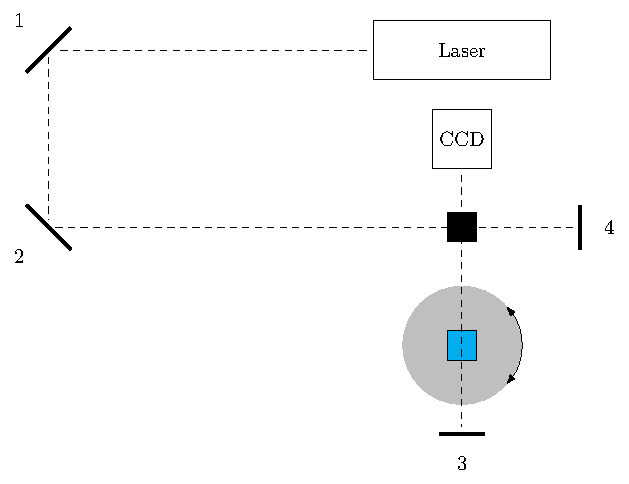
\includegraphics[width=0.5\textwidth]{img/schema.pdf}
    \caption{Apparatus scheme}
    \label{fig:ascheme}
\end{figure}
The experimental setting is similar to that of a Michelson-Morley interferometre with the addition of a liquid cuvette. It has the following components: 
\begin{itemize}
\item A LASER beam; %, whose wavelength is around \SI{532}{nm}; 
\item 4 mirrors, which are assumed to be perfectly reflective. Each mirror has two tiny handles, which are used to finely tilt the mirror with respect to the normal plane;
\item A beam splitter, which split the beam in two parts of similar intensity. The beam splitter has a support with tiny handles that allow you to tilt it with respect to the normal plane; 
\item A CCD, on which the beams interfere. It is capable of sending the interference picture to a PC. Some dampers have to be put in front of the CCD in order not to burn the pixels. Some examples of possible damping values are the following: $10^5$ when the beam is direcly pointed at the CCD (see step \ref{step:alignment} in the alignment section) and $10^3$ when the entire interferometre is working; 
\item A cuvette, made of glass. %, whose walls are approximately \SI{0.448}{cm} thick (nominal value).
 %glass. %, whose walls are approximately \SI{0.448}{cm} thick (nominal value).
Its walls should be of known thickness and very close to being parallel.
It has to be placed between the beam splitter and mirror 3 at the right height to have laser beam pass through the liquid;
\item A rotating support for the cuvette, which is moved by a step motor, controlled with an Arduino interface.
\end{itemize}

\section{Inteferometre Building and Alignment}
\begin{figure}[hbt]
    \centering
    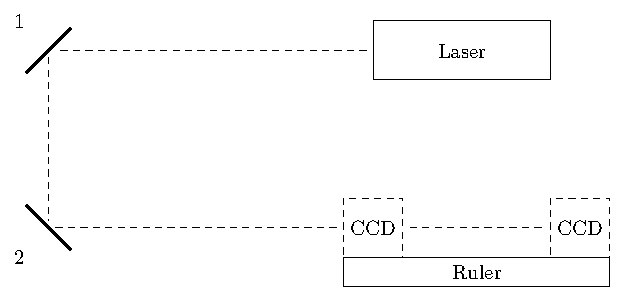
\includegraphics[width=0.5\textwidth]{img/align.pdf}
    \caption{First alignment steps.}
    \label{fig:align}
\end{figure}
The entire system has to be carefully aligned in order to have the two beams gather on the beam splitter and interfere on the CCD. The bulding of the interferometre should follow the steps below: 

\begin{enumerate}
    \item Place the laser in a fixed position on the optical bench and keep it fixed until the end of the experiment. Then, place mirror 1 and 2 in the positions that can be seen in the schematic in figure \ref{fig:align};
    \item  Rotate and tilt mirror 1 and mirror 2 so that the beam approximately points in the direction of the interferometre arm between mirror 2 and mirror 4;
    \item \label{step:alignment}Put the CCD on a movable support and build a guide that allows the CCD to move only on a fixed line, parallel to the interferometre arm between mirror 2 and 4. Then, choose two different positions along this line, which are far enough one from the other and iterate the following steps:
    \begin{itemize}
        \item Place the CCD in the position closer to mirror 2;
        \item Tilt mirror 1 on both axes, in order to have the beam in the centre of the CCD. To ease the process, the beam can be observed on the PC; %You would better look at the beam picture on the PC.
        \item Move the CCD in the position further from mirror 2;
        \item Tilt mirror 2 on both axes in order to have the beam in the centre of the CCD;
        \item Repeat the previous steps until you do not need to tilt mirrors anymore. 
    \end{itemize}
    \item Place mirror 4 in the position that can be seen in figure \ref{fig:ascheme}. Tilt mirror 4 in order to have the beam go back near the laser mouth but not into it;
    \item Place the beam splitter between mirror 2 and 4, then place mirror 3 and CCD;
    \item Tilt mirror 3 and beam splitter in order to have the two beams gather on the same spot both on the beam splitter and the CCD.
    \end{enumerate}
    
If the beams collide perfectly superimposed on the CCD, they interfere constructively or destructively creating a totally-on or a totally-off frame. It's useful to see intensity maximums and minimums moving through the frames: for this purpose, the beams can be slightly misaligned to produce interference fringes. The magnitude of the misalignment should be choosen to reach the best conditions; a good setup is the one with 3 fringes visible at a time.

\section{Rotating System}

In order to rotate the cuvette, put it on a rotating base equipped with a goniometre, coupled to a step motor with a belt, as shown if figure \ref{fig:top_view}.

\begin{figure}[H]
    \centering
    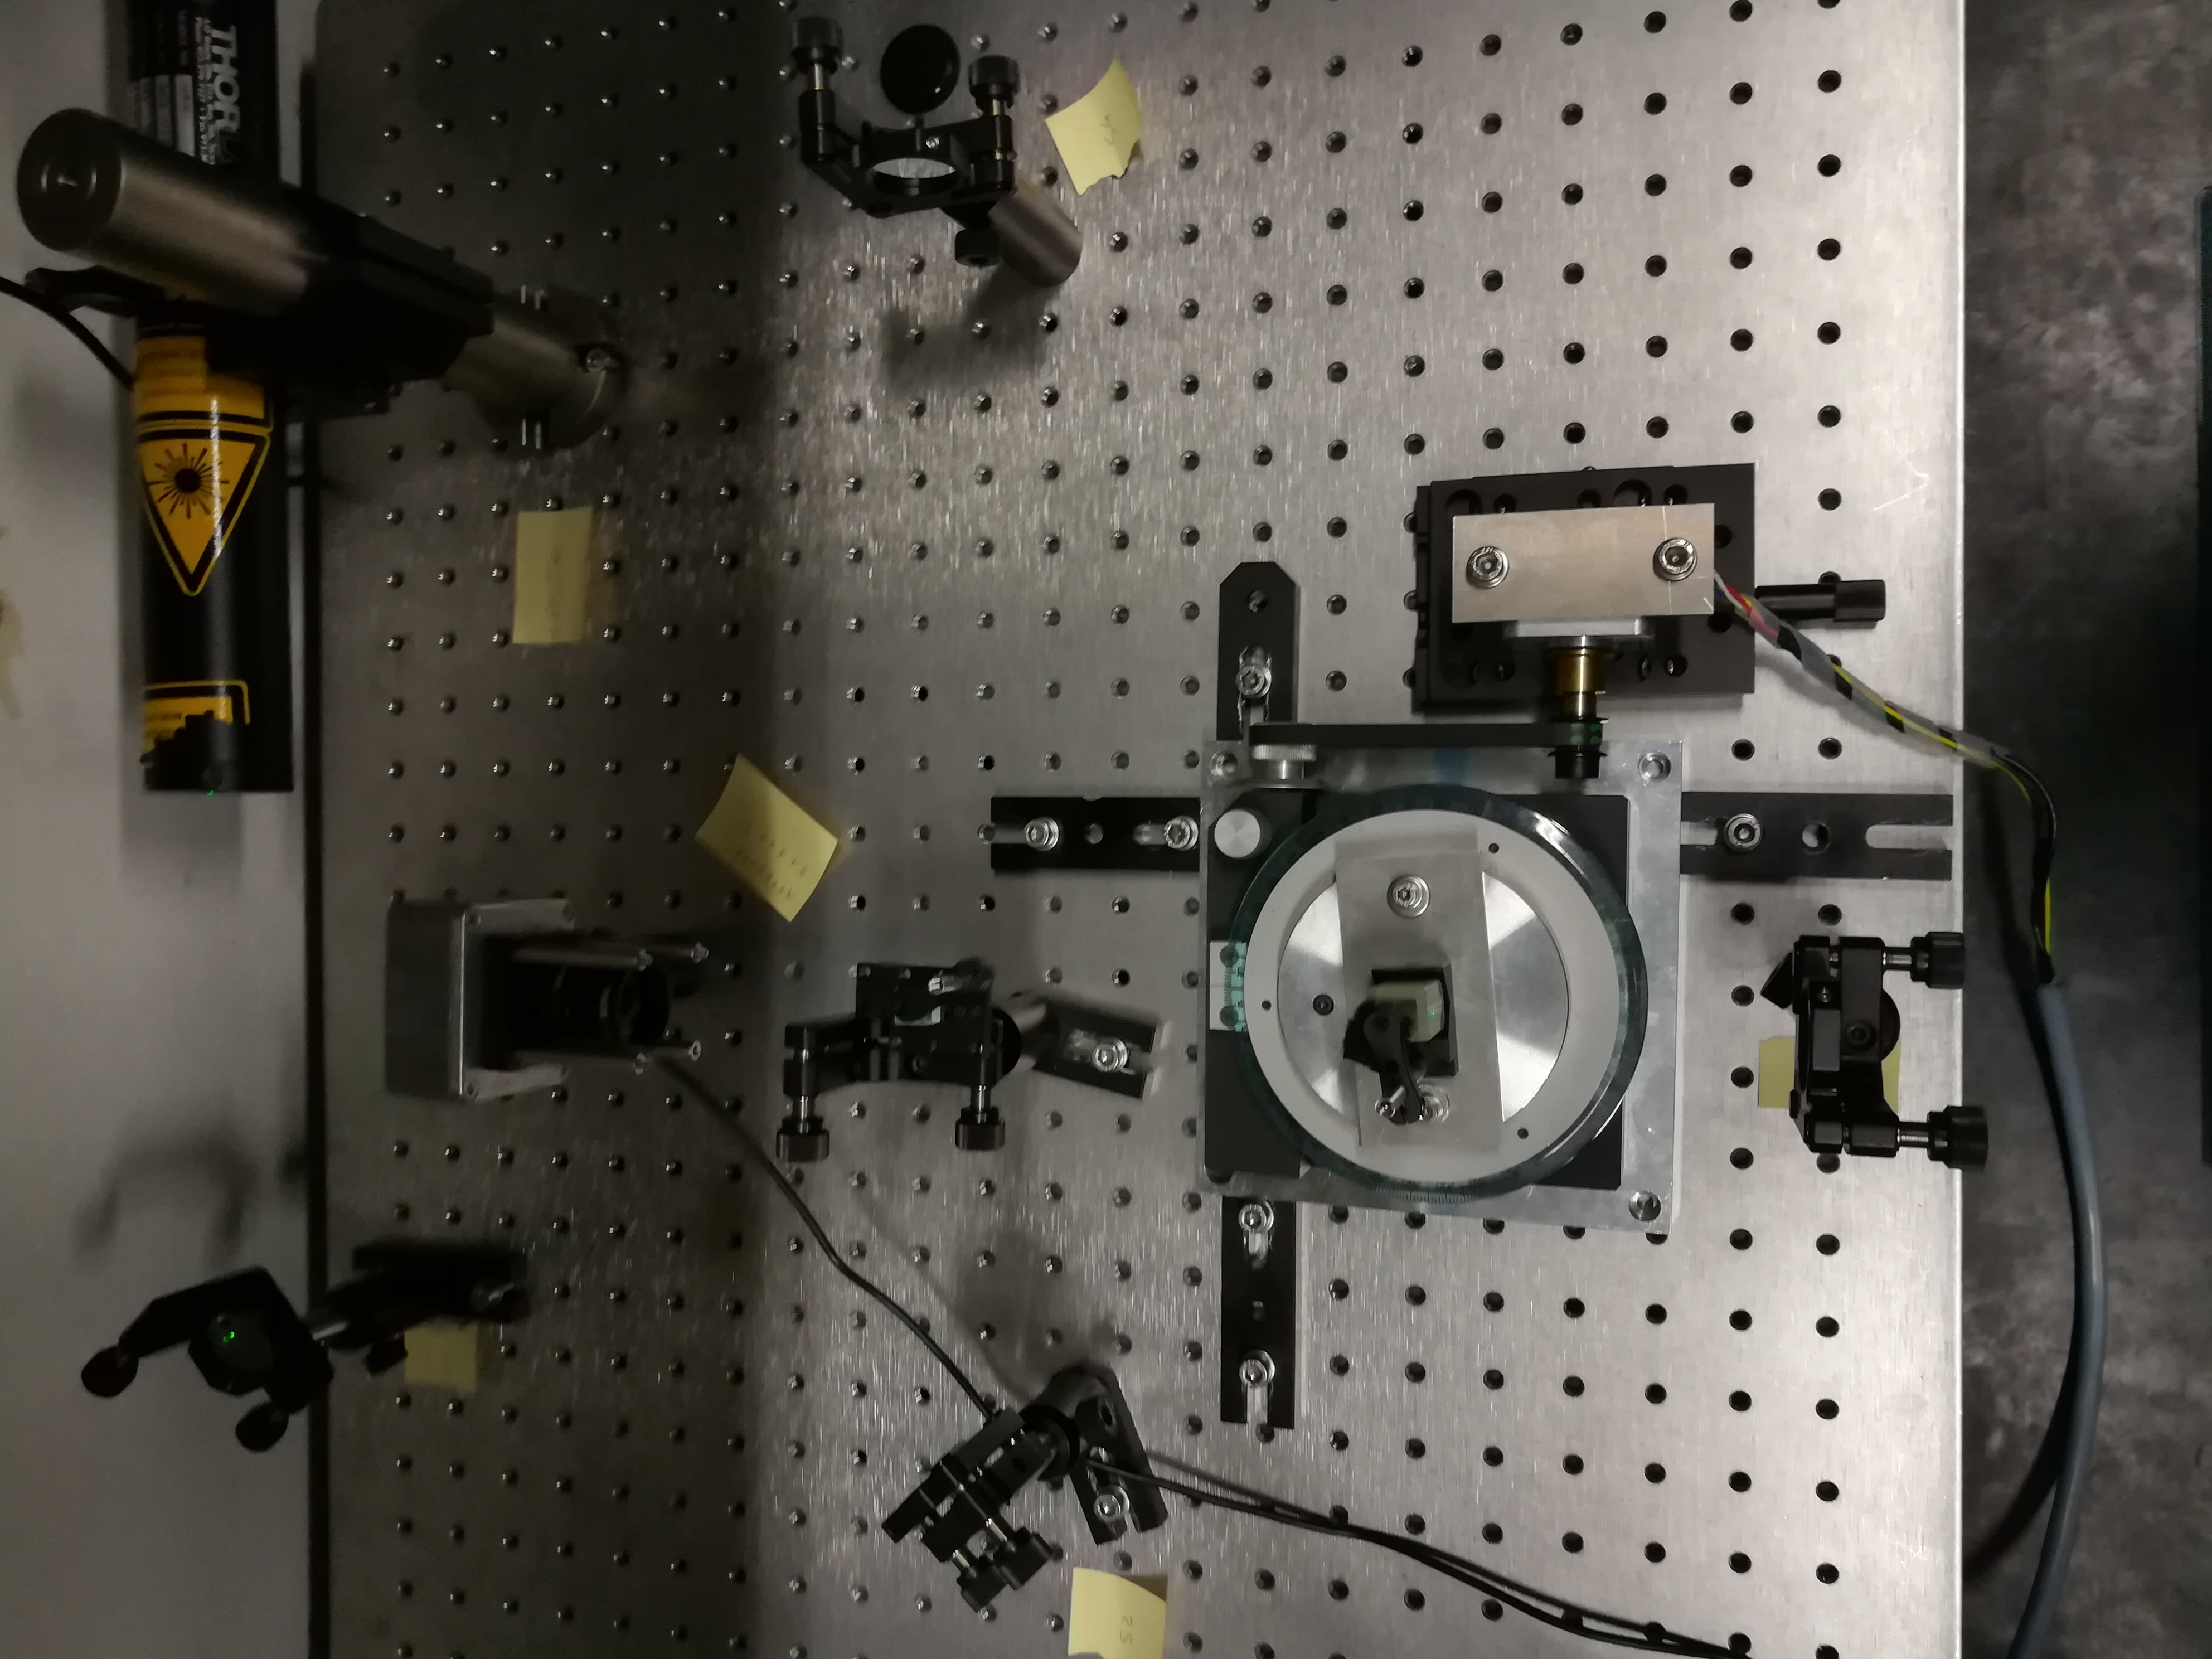
\includegraphics[width=0.4\textwidth]{img/motor_top_view.jpg}
    \caption{Motor placement}
    \label{fig:top_view}
\end{figure}

To secure the position of the rotating system base, which is not directly attachable to the optical bench, it is possible to use mirror supports on opposing sides.

Be sure to fix the motor firmly in place and to keep the belt taut to distribute the vibrations on the whole apparatus.

The step motor is driven by an Arduino board through a power supply.
Pay attention to the frequency of the step motor in order not to lose precision because of vibrations of the setup: you must be able to keep seeing the fringes on the CCD even with the motor running; a frequency of $\lesssim \SI{4}{Hz}$ should work.

\section{Step Motor Calibration}
Once the motor has been built, it is necessary to have a precise estimate of the conversion coefficient between steps and angles. 
It can be done through the following steps: 
\begin{itemize}
    \item Fix a goniometre on the base of the step motor, in order to measure in degrees the width of the motor rotation
    \item Every time the motor completes a one degree rotation, take note of the number of steps. Do not reset the step counter.
    \item Get the conversion coefficient, through a linear fit. It is reccomendable to have an estimate which has an error of the order of the $1 \%$ with respect to the value of the conversion coefficient.
\end{itemize}


%Measurements should be taken, first when the cuvette is empty and then when it is filled with liquid, for the simple reason that cuvette filling can be done, using a pipette, without changing the interferometre setting. Empting the cuvette, instead, requires us to to remove the cuvette from the rotating support.
%As a consequence, the background measurements are consistent only with the  measurement done, with the cuvette full of liquid, right after them. At the end, we had several signal measurements, obtained subtracting the background measurements to the corresponding background plus signal measurement.

%The operation of filling the cuvette with liquid is done with a pipette, so the system isn’t compromised. Instead, to empty the cuvette it is necessary to disassemble a part of the apparatus: the background measures are consistent only with the liquid measures taken just after them.
%So, before each liquid measure campaign, several background scans are done; then, the datasets considered for the signal computing and the fits are all the possible combinations between a background measure and a liquid measure.

\section{Theoretical Model}\label{sez:TM}

Using the Snell law of refraction and some basic geometrical rules, it is possible to obtain a formula which shows the dependance of the fringe order \(N\) with respect to the zero angle and the corresponding angle $\theta $, such that it is possible to split:

\begin{equation}
  N(\theta)_{\text{tot}}  =
  N(\theta)_{\text{background}}  +
  N(\theta)_{\text{signal}}
\end{equation}

By subtracting $N(\theta)_{\text{background}}$ (empty cuvette) from $N(\theta)_{\text{tot}}$ (full cuvette) it is possible to isolate the contribution from the liquid. 

Inverting the formula for $N(\theta)_{\text{signal}}$, it can be found that: 
\begin{equation}
\theta (N; \gamma, n_l, \theta_0, N_0 )
=\theta_0  +
\operatorname{sgn}(N) \operatorname{arccos}\qty(\frac{
n_l^2-1-\qty(\gamma \qty(\abs{N}-N_0) + n_l - 1)^2
}{
2 \qty(\gamma \qty(\abs{N}-N_0)+n_l -1)
})
\end{equation}

where \(N\) is the number of the fringe, \(n_l\) is the liquid refractive index and \(\gamma\) is
a parameter depending on the cuvette width \(d\) and the laser wavelength $\gamma = \frac{\lambda}{2d}$.
Since the zero positions are not well known neither for \(\theta\) nor for \(N\), two offset parameters must be added: \(\theta\) is replaced with \(\theta - \theta_0\) and \(N\) with \(N-N_0\). Finally, a module and a sign function are added in order to consider negative-order fringes.

Furthermore, if we consider the $N(\theta)$ formula for small $\theta$, we get:

\begin{equation}
    N(\theta) \sim
    \theta^{2} \left(\frac{1}{2 \gamma} - \frac{1}{2 \gamma n_l}\right) + \theta^{4} \left(- \frac{1}{24 \gamma} + \frac{1}{6 \gamma n_l} - \frac{1}{8 \gamma n^{3}_l}\right) + O\left(\theta^{6}\right)
\end{equation}

the second-order term can be rewritten as $\theta^2 (n_l-1) / (2\gamma n_l)$: different values of $n_l$ and $\gamma$ give the same prediction up to third order as long as they have the same value of $(n_l-1) / (2\gamma n_l)$. For the ranges of values which will be used to fit later the contour lines of this relation are almost linear.

\section{Collecting measurements}
At this point it is possible to take measurements, with the following protocol: 
\begin{enumerate}
\item Place the empty cuvette on the support and turn the support at about $7\divisionsymbol \SI{8}{\degree}$ from the position where the cuvette is orthogonal to the beam; 
\item Turn on the step motor and start the acquisition of the interference pattern until the cuvette reaches $7\divisionsymbol \SI{8}{\degree}$ on the other side; 
\item Acquire three/four background datasets, all in the same experimental conditions, without touching the cuvette or anything in the interferometre; 
\item Using a pipette, fill with extreme caution the cuvette with the liquid. Acquire three or four datasets with the liquid; 

\end{enumerate}

It is important to note that when the liquid is removed from the cuvette, the cuvette itself has to be taken away from the support and the experimental conditions are inevitably altered. Therefore the background measurements are consistent only with the liquid measures taken just after them.

Since $\gamma$ and $n_l$ are strongly correlated - as shown in \ref{sez:TM} - it is impossible to estimate them simultaneously with only one dataset. Hence, first use a liquid whose refractive index is well known (i.e. water) in order to get the value of $\gamma$. Then you can take measurements with the liquid, whose refraction index you have to estiamate.

\section{Our data analysis code}
The code for the analysis can be found at \url{https://github.com/jacopok/interferometry}. It is mainly divided into five parts:

\begin{enumerate}
    \item \textbf{data gathering}: stepper motor management, sensor management, data collection; \label{step:gathering}
    \item \textbf{dataset generation}: minimum search, generation of fringe-step dataset files; \label{step:generation}
    \item \textbf{dataset management}: preliminary fitting, centering of datasets, subtraction and error propagation, generation of error PDFs; \label{step:management}
    \item \textbf{fitting}: Montecarlo maximum-likelihood fitting of datasets with variable parameters; \label{step:fitting}
    \item \textbf{result synthesis}: dataset and PDF plotting, averaging of PDFs. \label{step:synthesis}
\end{enumerate}

The code for step \ref{step:gathering} is in the folder \lstinline{applicativo}. It's a root-based c++ program, which uses the \lstinline{opencv} libraries. It's splitted in four classes: \lstinline{spokeperson} manage the communications with arduino and ccd, \lstinline{GUI} the main graphical interface, \lstinline{analisi} and \lstinline{biggraph} the computation and showing of the minimuns. This first minimums computation it's only approximative and it's useful to be sure that, during acquisition, everything is working properly. They must be recomputed when the signal is totally available and the thresholds can be properly setted.

The code for step \ref{step:generation} can be found in the folder \lstinline{/data/Minsfinder}. The data must be watched and the best threshold must be choosen, then an a-posteriori minimums computation must be done.

The code for step \ref{step:management} is mainly managed in the file \lstinline{Fringes_dataset_manager.py}. An instance of the class \lstinline{dataset} corresponds to a single measurement (in which the cuvette is rotated from an angle to another).
An instance of the class \lstinline{measure} corresponds to a background-gross signal pair, and it is where the subtraction is performed.

These classes are utilized in the functions in \lstinline{initialization.py} which in turn are called in the script \lstinline{process_data.py}, which outputs all the background-subtracted files in a format which the programs in \lstinline{/montecarlo/} can understand. The \lstinline{process_data.py} script outputs the weighted half-widths of the triangular distributions to convolve, and the script at \lstinline{/montecarlo/Sources/QbicFactory.cc} generates the third order distributions corresponding to the convolution of triangulars.

The code for step \ref{step:fitting} can be found in the directory \lstinline{/montecarlo/}. Instructions for usage are contained in \lstinline{How_to_use.txt}.

Regarding step \ref{step:synthesis}: the code for the calculation of the average of several PDFs can be found at \lstinline{/montecarlo/Gamma/average.cxx};
the code used for figure generation is gathered in the script \lstinline{figure_generator.py}, which uses the functions in \lstinline{PDF_reader.py} to read the one-dimensional and multi-dimensional PDFs.

\end{document}